\documentclass{ThesisStyle}
\selectlanguage{english}
%\usepackage{amsmath,amssymb,amscd,mathrsfs}
%\usepackage[mathscr]{euscript}
\usepackage{xspace}
\usepackage[binary-units=true]{siunitx}
\usepackage{lineno}
\usepackage{graphicx}
\usepackage{feynmp-auto}
\usepackage{float}
\usepackage{scalerel}
\usepackage{tikz}
\usepackage{tikz-3dplot}
\tikzset{>=latex} % for LaTeX arrow head

\newcommand{\mybrace}[1]{\scaleleftright[\dimexpr6pt+#1\dimexpr0.11pt]{.}{\rule[\dimexpr5pt-#1\dimexpr0.5pt]{-4pt}{#1pt}}{\rbrace}\hspace{-1pt}}

\DeclareRobustCommand{\euscr}[1]{\text{\usefont{U}{eus}{m}{n}#1}}
\DeclareSIUnit{\Bit}{b}

\usepackage{titlesec}
\usepackage{etoolbox}
\titleclass{\subsubsubsection}{straight}[\subsubsection]
\newcounter{subsubsubsection}[subsubsection]
\renewcommand\thesubsubsubsection{\thesubsubsection.\arabic{subsubsubsection}}
\renewcommand\theparagraph{\thesubsubsubsection.\arabic{paragraph}}
\titleformat{\subsubsubsection}{\normalfont\normalsize\bfseries}{\thesubsubsubsection}{1em}{}
\titlespacing*{\subsubsubsection}{0pt}{3.25ex plus 1ex minus .2ex}{1.5ex plus .2ex}
\makeatletter
\renewcommand\paragraph{\@startsection{paragraph}{5}{\z@}{3.25ex \@plus1ex \@minus.2ex}{-1em}{\normalfont\normalsize\bfseries}}
\renewcommand\subparagraph{\@startsection{subparagraph}{6}{\parindent}{3.25ex \@plus1ex \@minus .2ex}{-1em}{\normalfont\normalsize\bfseries}}
\def\toclevel@subsubsubsection{4}
\def\toclevel@paragraph{5}
\def\toclevel@subparagraph{6}
\def\l@subsubsubsection{\@dottedtocline{4}{7em}{4em}}
\def\l@paragraph{\@dottedtocline{5}{10em}{5em}}
\def\l@subparagraph{\@dottedtocline{6}{14em}{6em}}
\makeatother
\makeatletter
\patchcmd{\ttlh@hang}{\parindent\z@}{\parindent\z@\leavevmode}{}{}
\patchcmd{\ttlh@hang}{\noindent}{}{}{}
\makeatother
\setcounter{secnumdepth}{4}
\setcounter{tocdepth}{4}

\begin{document}

%%%%%%%%%%%%%% W ANALYSIS %%%%%%%%%%%%%%%%%%%%%%%%%%%%%%%%%%%%%%%

% Analysis Observables
\newcommand{\ChgAsym}{{\cal C}\xspace}
\newcommand{\RFB}{\ensuremath{\text{R}_\text{FB}}\xspace}
\newcommand{\RFBp}{\ensuremath{\text{R}_\text{FB}^+}\xspace}
\newcommand{\RFBm}{\ensuremath{\text{R}_\text{FB}^-}\xspace}

% Physics Particles and Decays
\newcommand{\PW}{\ensuremath{\text{W}}}
\newcommand{\PWp}{\ensuremath{\text{W}^{+}}}
\newcommand{\PWm}{\ensuremath{\text{W}^{-}}}
\newcommand{\PWpm}{\ensuremath{\text{W}^{\pm}}}
\newcommand{\PZ}{\ensuremath{\text{Z}}\xspace}
\newcommand{\PGm}{\ensuremath{\mu}\xspace} % muon
\newcommand{\PGmm}{\ensuremath{\mu^-}\xspace} % muon
\newcommand{\PGmp}{\ensuremath{\mu^+}\xspace} % muon
\newcommand{\PGmpm}{\ensuremath{\mu^\pm}\xspace} % muon
\newcommand{\PGn}{\ensuremath{\nu}\xspace} % generic neutrino
\newcommand{\PAGn}{\ensuremath{\overline{\nu}}\xspace} % generic neutrino
\newcommand{\PGnl}{\ensuremath{\nu_\text{l}}\xspace} % lepton neutrino
\newcommand{\PAGnl}{\ensuremath{\overline{\nu}_\text{l}}\xspace} % anti-lepton neutrino
\newcommand{\PGnGm}{\ensuremath{\nu_\PGm}\xspace} % muon neutrino
\newcommand{\PAGnGm}{\ensuremath{\overline{\nu}_\PGm}\xspace} % anti-muon neutrinoPsi
\newcommand{\PGnGt}{\ensuremath{\nu_\PGt}\xspace} % tau neutrino
\newcommand{\PAGnGt}{\ensuremath{\overline{\nu}_\PGt}\xspace} % anti-tau neutrino
\newcommand{\PGt}{\ensuremath{\tau}\xspace} % tau
\newcommand{\PAGt}{\ensuremath{\overline{\tau}}\xspace} % anti-tau
\newcommand{\PQt}{\ensuremath{\text{t}}\xspace} % t
\newcommand{\PQb}{\ensuremath{\text{b}}\xspace} % b
\newcommand{\cPqu}{\ensuremath{\text{u}}} % u for u quark
\newcommand{\cPqd}{\ensuremath{\text{d}}} % d for d quark
\newcommand{\cPaqu}{\ensuremath{\overline{\text{u}}}} % u for u quark
\newcommand{\cPaqd}{\ensuremath{\overline{\text{d}}}} % d for d quark
%%
\newcommand{\mumu}{\ensuremath{\PGmp\PGmm}\xspace}
\newcommand{\tautau}{\ensuremath{\PGt\PAGt}\xspace}
\newcommand{\Wb}{\ensuremath{\PW}\xspace}
\newcommand{\Wp}{\ensuremath{\PWp}\xspace}
\newcommand{\Wm}{\ensuremath{\PWm}\xspace}
\newcommand{\Wpm}{\ensuremath{\PWpm}\xspace}
\newcommand{\DY}{\ensuremath{\PZ/\gamma*}\xspace} % Drell-Yan
\newcommand{\DYToMuMu}{\ensuremath{\DY\to\mumu}\xspace}
\newcommand{\Z}{\ensuremath{\PZ}\xspace}
\newcommand{\ZToMuMu}{\ensuremath{\Z\to\mumu}\xspace}
\newcommand{\DYToTauTau}{\ensuremath{\DY\to\tautau}\xspace}
\newcommand{\ZToTauTau}{\ensuremath{\Z\to\tautau}\xspace}
\newcommand{\WToMuNu}{\ensuremath{\Wb\to\PGm\PGnGm}\xspace}
\newcommand{\WToMuNuPl}{\ensuremath{\PWp\to\PGmp\PGnGm}\xspace}
\newcommand{\WToMuNuMi}{\ensuremath{\PWm\to\PGmm\PAGnGm}\xspace}
\newcommand{\WToTauNu}{\ensuremath{\Wb\to\PGt\PGnGt}\xspace}
\newcommand{\WToTauNuPl}{\ensuremath{\PWp\to\PAGt\PGnGt}\xspace}
\newcommand{\WToTauNuMi}{\ensuremath{\PWm\to\PGt\PAGnGt}\xspace}
\newcommand{\ttbar}{\ensuremath{\text{t}\overline{\text{t}}}\xspace} % t-tbar
\newcommand{\QQbar}{\ensuremath{{\text{Q}\overline{\text{Q}}}}\xspace}
\newcommand{\JPsi}{\ensuremath{\text{J}\hspace{-.08em}/\hspace{-.14em}\psi}\xspace} % J/Psi (no mass)
\newcommand{\PsiOneS}{\ensuremath{\psi\left(2\text{S}\right)}\xspace}
\newcommand{\UpsOneS}{\ensuremath{\Upsilon\left(1\text{S}\right)}\xspace}
\newcommand{\UpsTwoS}{\ensuremath{\Upsilon\left(2\text{S}\right)}\xspace}
\newcommand{\UpsThreeS}{\ensuremath{\Upsilon\left(3\text{S}\right)}\xspace}
\newcommand{\B}{\ensuremath{\text{B}}\xspace}
\newcommand{\D}{\ensuremath{\text{D}}\xspace}

% Collision Types
\newcommand{\Pp}{\ensuremath{\text{p}}}
\newcommand{\Pb}{\ensuremath{\text{Pb}}\xspace}
\newcommand{\pp}{{\ensuremath{\Pp\Pp}}\xspace}
\newcommand{\pn}{{\ensuremath{{\Pp}n}}\xspace}
\newcommand{\pPb}{\ensuremath{\Pp\text{Pb}}\xspace}
\newcommand{\Pbp}{\ensuremath{\text{Pb}\Pp}\xspace}
\newcommand{\RunpPb}{\ensuremath{\Pp\text{-}\Pb}\xspace}
\newcommand{\RunPbp}{\ensuremath{\Pb\text{-}\Pp}\xspace}
\newcommand{\RunPbPb}{\ensuremath{\Pb\text{-}\Pb}\xspace}
\newcommand{\Runpp}{\ensuremath{\Pp\text{-}\Pp}\xspace}
\newcommand{\RunXeXe}{\ensuremath{\mathrm{Xe}\text{-}\mathrm{Xe}}\xspace}
\newcommand{\RunpA}{\ensuremath{\Pp\text{-}\text{A}}\xspace}

% Physics Units
%\newcommand{\TeV}{\ensuremath{\,\text{Te\hspace{-.08em}V}}\xspace}
%\newcommand{\MeV}{\ensuremath{\,\text{Me\hspace{-.08em}V}}\xspace}
%\newcommand{\GeV}{\ensuremath{\,\text{Ge\hspace{-.08em}V}}\xspace}
\newcommand{\GeVc}{\ensuremath{{\,\text{Ge\hspace{-.08em}V\hspace{-0.16em}/\hspace{-0.08em}}c}}\xspace}
\newcommand{\GeVcc}{\ensuremath{{\,\text{Ge\hspace{-.08em}V\hspace{-0.16em}/\hspace{-0.08em}}c^\text{2}}}\xspace}
\newcommand{\nbinv} {\mbox{\ensuremath{\,\text{nb}^\text{$-$1}}}\xspace}

% Physics Symbols ...
\newcommand{\etaLAB}{\ensuremath{\eta_{\mathrm{lab}}}\xspace}
\newcommand{\etaCM}{\ensuremath{\eta_{\mathrm{CM}}}\xspace}
\newcommand{\pt}{\ensuremath{p_{\mathrm{T}}}\xspace}
\newcommand{\Et}{\ensuremath{E_{\mathrm{T}}}\xspace}
\newcommand{\Em}{\ensuremath{E\hspace{-0.6em}/}\xspace}
\newcommand{\ETm}{\ensuremath{E_{\mathrm{T}}^{\text{miss}}}\xspace}
\newcommand{\MET}{\ETm}
\newcommand{\ETmiss}{\ETm}
\newcommand{\ptmiss}{\ensuremath{\pt^\text{miss}}\xspace}
\newcommand{\ETslash}{\ensuremath{E_{\mathrm{T}}\hspace{-1.1em}/\kern0.45em}\xspace}
\newcommand{\VETslash}{\ensuremath{{\vec E}_{\mathrm{T}}\hspace{-1.1em}/\kern0.45em}\xspace}
\newcommand{\VEtmiss}{\ensuremath{{\vec E}_{\mathrm{T}}^{\text{miss}}}\xspace}
\newcommand{\ptvec}{\ensuremath{{\vec p}_{\mathrm{T}}}\xspace}
\newcommand{\ptvecmiss}{\ensuremath{{\vec p}_{\mathrm{T}}^{\kern1pt\text{miss}}}\xspace}
\newcommand{\sqrts}{\ensuremath{\sqrt{\smash[b]{s}}}\xspace}
\newcommand{\sqrtsnn}{\ensuremath{\sqrt{\smash[b]{s_{_{\mathrm{NN}}}}}}\xspace}
\newcommand{\snn}{\ensuremath{\smash[b]{s_{_{\mathrm{NN}}}}}\xspace}
\newcommand{\Lumi}{\ensuremath{\mathrm{L}}\xspace}%both upper and lower % FIX WITH MATHCAL

% Software Programs
\newcommand{\CMSSW} {{\textsc{cmssw}}\xspace}
\newcommand{\EVTGEN} {{\textsc{evtgen}}\xspace}
\newcommand{\FEWZ} {{\textsc{fewz}}\xspace}
\newcommand{\GEANTfour} {{\textsc{Geant4}}\xspace}
\newcommand{\GEANT} {{\textsc{geant}}\xspace}
\newcommand{\POWHEG} {{\textsc{powheg}}\xspace}
\newcommand{\HIJING} {{\textsc{hijing}}\xspace}
\newcommand{\HYDJET} {{\textsc{hydjet}}\xspace}
\newcommand{\MCFM} {\textsc{mcfm}\xspace}
\newcommand{\PHOTOS} {\textsc{photos}\xspace}
\newcommand{\PYTHIA} {{\textsc{pythia}}\xspace}
\newcommand{\TAUOLA} {\textsc{tauola}\xspace}
\newcommand{\POWHEGBOX} {{\textsc{powheg}}-{\textsc{box}}\xspace}
\newcommand{\EPOS} {{\textsc{epos}}\xspace}
\newcommand{\PYQUEN} {{\textsc{pyquen}}\xspace}

% Operators
\newcommand{\abs}[1]{\ensuremath{\lvert #1 \rvert}}
\newcommand{\eexp}[1]{\ensuremath{{\text e}^{#1}}\xspace}

% References to Equations, Figures, Tables, Sections or Chapters
\newcommand{\eq}[1]{Eq.~\eqref{#1}\xspace}
\newcommand{\fig}[1]{Fig.~\ref{#1}\xspace}
\newcommand{\tab}[1]{Table~\ref{#1}\xspace}
\newcommand{\sect}[1]{Section~\ref{#1}\xspace}
\newcommand{\chp}[1]{Chapter~\ref{#1}\xspace}


%------------------------------------------------------------------------------

%%%%%%%%%%% COVER
\frontmatter
\pagenumbering{roman}


\includepdf[pages=1-]{Cover/Cover.pdf}
\clearemptydoublepage

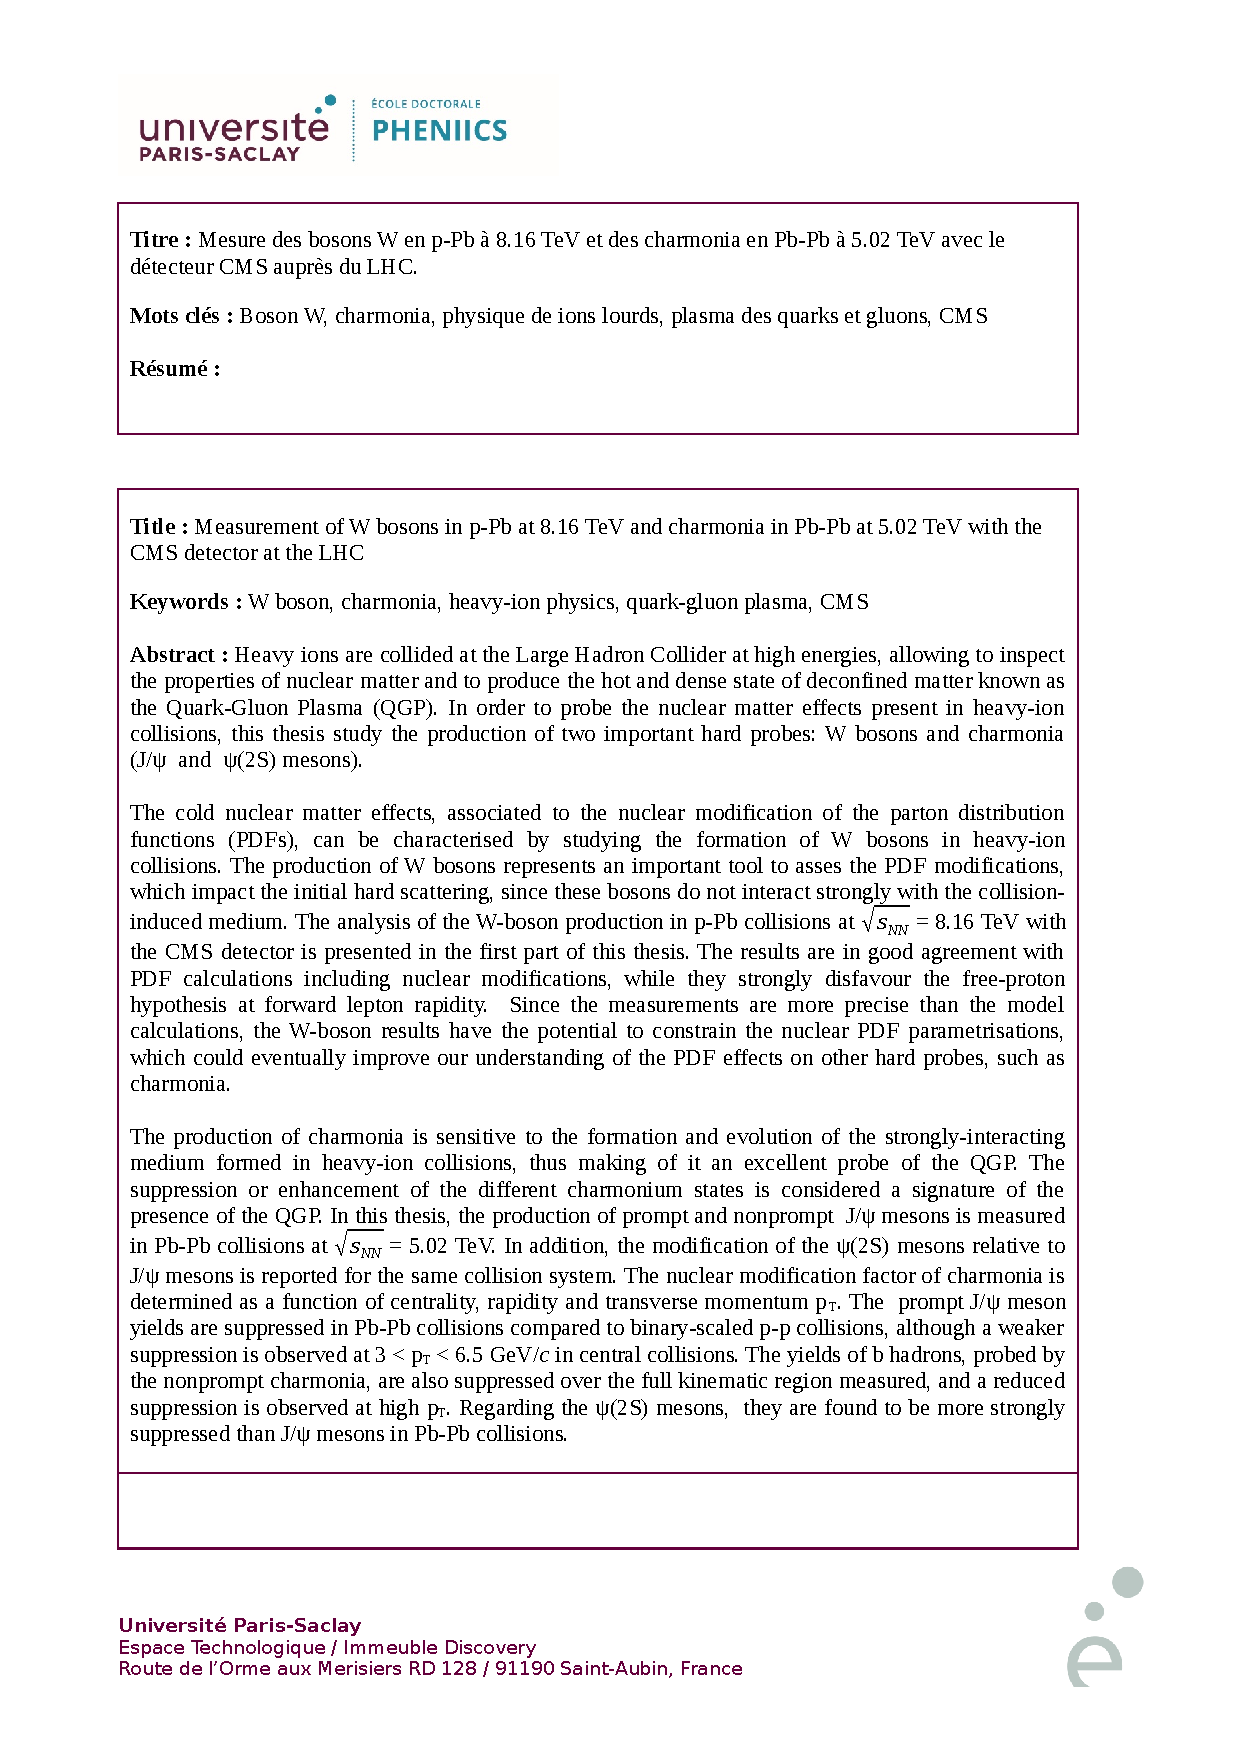
\includepdf[pages=1-]{Cover/Abstract.pdf}
\clearemptydoublepage

%\includepdf[pages=1-]{frontmatter/Acknowledgements.pdf}
%\clearemptydoublepage


%------------------------------------------------------------------------------

%%%%%%%%%%% TABLE OF CONTENTS
\renewcommand{\contentsname}{Table of Contents}
\maxtocdepth{subsection}
\tableofcontents
\addtocontents{toc}{\par\nobreak \mbox{}\hfill{\textbf{Page}}\par\nobreak}
\clearemptydoublepage


%------------------------------------------------------------------------------

%%%%%%%%%%% CHAPTERS
\mainmatter

\begin{linenumbers}

\import{Chapters/Main/Introduction/}{Chapter.tex}
\clearemptydoublepage

\import{Chapters/Main/Experiment/}{Chapter.tex}
\clearemptydoublepage

\import{Chapters/Main/WBoson/}{Chapter.tex}
\clearemptydoublepage

\import{Chapters/Main/Charmonia/}{Chapter.tex}
\clearemptydoublepage

\import{Chapters/Main/Conclusion/}{Chapter.tex}
\clearemptydoublepage

\end{linenumbers}


%------------------------------------------------------------------------------

%%%%%%%%%%% APPENDIX
\appendix

\import{Chapters/Appendix/WBoson/SignalExtraction/}{Fits.tex}
\clearemptydoublepage

\import{Chapters/Appendix/Charmonia/}{Binning.tex}
\clearemptydoublepage


%%Change the geometry for signal extraction plots
%\newgeometry{margin=1cm,includefoot}
%\restoregeometry
%%%%%%%%%%%%%%%%%%%%%%%%%%%%%%%


%------------------------------------------------------------------------------

%%%%%%%%%%% BIBLIOGRAPHY
\backmatter
\bibliographystyle{kp}
\bibliography{Bibliography/Introduction,Bibliography/Experiment,Bibliography/WBoson_Theory,Bibliography/WBoson_Analysis,Bibliography/Charmonia_Theory,Bibliography/Charmonia_Analysis}
\clearemptydoublepage


%------------------------------------------------------------------------------

%%%%%%%%%%% LIST OF FIGURES AND TABLES
\clearemptydoublepage
\listoftables
\addtocontents{lot}{\par\nobreak\textbf{{\scshape Table} \hfill Page}\par\nobreak}


\clearemptydoublepage
\listoffigures
\addtocontents{lof}{\par\nobreak\textbf{{\scshape Figure} \hfill Page}\par\nobreak}
\clearemptydoublepage


% END OF THESIS
\end{document}
